\documentclass[]{article}
\usepackage{lmodern}
\usepackage{amssymb,amsmath}
\usepackage{ifxetex,ifluatex}
\usepackage{fixltx2e} % provides \textsubscript
\ifnum 0\ifxetex 1\fi\ifluatex 1\fi=0 % if pdftex
  \usepackage[T1]{fontenc}
  \usepackage[utf8]{inputenc}
\else % if luatex or xelatex
  \ifxetex
    \usepackage{mathspec}
  \else
    \usepackage{fontspec}
  \fi
  \defaultfontfeatures{Ligatures=TeX,Scale=MatchLowercase}
\fi
% use upquote if available, for straight quotes in verbatim environments
\IfFileExists{upquote.sty}{\usepackage{upquote}}{}
% use microtype if available
\IfFileExists{microtype.sty}{%
\usepackage{microtype}
\UseMicrotypeSet[protrusion]{basicmath} % disable protrusion for tt fonts
}{}
\usepackage[margin=1in]{geometry}
\usepackage{hyperref}
\hypersetup{unicode=true,
            pdftitle={Mentor Work Sample for Practical Machine Learning: Predicting Activity Quality Based on Weight Lifting Exercise Data},
            pdfauthor={Kunyu He},
            pdfborder={0 0 0},
            breaklinks=true}
\urlstyle{same}  % don't use monospace font for urls
\usepackage{color}
\usepackage{fancyvrb}
\newcommand{\VerbBar}{|}
\newcommand{\VERB}{\Verb[commandchars=\\\{\}]}
\DefineVerbatimEnvironment{Highlighting}{Verbatim}{commandchars=\\\{\}}
% Add ',fontsize=\small' for more characters per line
\usepackage{framed}
\definecolor{shadecolor}{RGB}{248,248,248}
\newenvironment{Shaded}{\begin{snugshade}}{\end{snugshade}}
\newcommand{\KeywordTok}[1]{\textcolor[rgb]{0.13,0.29,0.53}{\textbf{#1}}}
\newcommand{\DataTypeTok}[1]{\textcolor[rgb]{0.13,0.29,0.53}{#1}}
\newcommand{\DecValTok}[1]{\textcolor[rgb]{0.00,0.00,0.81}{#1}}
\newcommand{\BaseNTok}[1]{\textcolor[rgb]{0.00,0.00,0.81}{#1}}
\newcommand{\FloatTok}[1]{\textcolor[rgb]{0.00,0.00,0.81}{#1}}
\newcommand{\ConstantTok}[1]{\textcolor[rgb]{0.00,0.00,0.00}{#1}}
\newcommand{\CharTok}[1]{\textcolor[rgb]{0.31,0.60,0.02}{#1}}
\newcommand{\SpecialCharTok}[1]{\textcolor[rgb]{0.00,0.00,0.00}{#1}}
\newcommand{\StringTok}[1]{\textcolor[rgb]{0.31,0.60,0.02}{#1}}
\newcommand{\VerbatimStringTok}[1]{\textcolor[rgb]{0.31,0.60,0.02}{#1}}
\newcommand{\SpecialStringTok}[1]{\textcolor[rgb]{0.31,0.60,0.02}{#1}}
\newcommand{\ImportTok}[1]{#1}
\newcommand{\CommentTok}[1]{\textcolor[rgb]{0.56,0.35,0.01}{\textit{#1}}}
\newcommand{\DocumentationTok}[1]{\textcolor[rgb]{0.56,0.35,0.01}{\textbf{\textit{#1}}}}
\newcommand{\AnnotationTok}[1]{\textcolor[rgb]{0.56,0.35,0.01}{\textbf{\textit{#1}}}}
\newcommand{\CommentVarTok}[1]{\textcolor[rgb]{0.56,0.35,0.01}{\textbf{\textit{#1}}}}
\newcommand{\OtherTok}[1]{\textcolor[rgb]{0.56,0.35,0.01}{#1}}
\newcommand{\FunctionTok}[1]{\textcolor[rgb]{0.00,0.00,0.00}{#1}}
\newcommand{\VariableTok}[1]{\textcolor[rgb]{0.00,0.00,0.00}{#1}}
\newcommand{\ControlFlowTok}[1]{\textcolor[rgb]{0.13,0.29,0.53}{\textbf{#1}}}
\newcommand{\OperatorTok}[1]{\textcolor[rgb]{0.81,0.36,0.00}{\textbf{#1}}}
\newcommand{\BuiltInTok}[1]{#1}
\newcommand{\ExtensionTok}[1]{#1}
\newcommand{\PreprocessorTok}[1]{\textcolor[rgb]{0.56,0.35,0.01}{\textit{#1}}}
\newcommand{\AttributeTok}[1]{\textcolor[rgb]{0.77,0.63,0.00}{#1}}
\newcommand{\RegionMarkerTok}[1]{#1}
\newcommand{\InformationTok}[1]{\textcolor[rgb]{0.56,0.35,0.01}{\textbf{\textit{#1}}}}
\newcommand{\WarningTok}[1]{\textcolor[rgb]{0.56,0.35,0.01}{\textbf{\textit{#1}}}}
\newcommand{\AlertTok}[1]{\textcolor[rgb]{0.94,0.16,0.16}{#1}}
\newcommand{\ErrorTok}[1]{\textcolor[rgb]{0.64,0.00,0.00}{\textbf{#1}}}
\newcommand{\NormalTok}[1]{#1}
\usepackage{longtable,booktabs}
\usepackage{graphicx,grffile}
\makeatletter
\def\maxwidth{\ifdim\Gin@nat@width>\linewidth\linewidth\else\Gin@nat@width\fi}
\def\maxheight{\ifdim\Gin@nat@height>\textheight\textheight\else\Gin@nat@height\fi}
\makeatother
% Scale images if necessary, so that they will not overflow the page
% margins by default, and it is still possible to overwrite the defaults
% using explicit options in \includegraphics[width, height, ...]{}
\setkeys{Gin}{width=\maxwidth,height=\maxheight,keepaspectratio}
\IfFileExists{parskip.sty}{%
\usepackage{parskip}
}{% else
\setlength{\parindent}{0pt}
\setlength{\parskip}{6pt plus 2pt minus 1pt}
}
\setlength{\emergencystretch}{3em}  % prevent overfull lines
\providecommand{\tightlist}{%
  \setlength{\itemsep}{0pt}\setlength{\parskip}{0pt}}
\setcounter{secnumdepth}{5}
% Redefines (sub)paragraphs to behave more like sections
\ifx\paragraph\undefined\else
\let\oldparagraph\paragraph
\renewcommand{\paragraph}[1]{\oldparagraph{#1}\mbox{}}
\fi
\ifx\subparagraph\undefined\else
\let\oldsubparagraph\subparagraph
\renewcommand{\subparagraph}[1]{\oldsubparagraph{#1}\mbox{}}
\fi

%%% Use protect on footnotes to avoid problems with footnotes in titles
\let\rmarkdownfootnote\footnote%
\def\footnote{\protect\rmarkdownfootnote}

%%% Change title format to be more compact
\usepackage{titling}

% Create subtitle command for use in maketitle
\newcommand{\subtitle}[1]{
  \posttitle{
    \begin{center}\large#1\end{center}
    }
}

\setlength{\droptitle}{-2em}
  \title{Mentor Work Sample for Practical Machine Learning: Predicting Activity
Quality Based on Weight Lifting Exercise Data}
  \pretitle{\vspace{\droptitle}\centering\huge}
  \posttitle{\par}
  \author{Kunyu He}
  \preauthor{\centering\large\emph}
  \postauthor{\par}
  \predate{\centering\large\emph}
  \postdate{\par}
  \date{22 June 2018}


\begin{document}
\maketitle

\section{Executive Summary}\label{executive-summary}

One thing that people regularly do, using devices such as \emph{Jawbone
Up}, \emph{Nike FuelBand}, and \emph{Fitbit} to take measurements of
their activities regularly, is to quantify how much of a particular
activity they do, but they rarely quantify how well they do it.

In this project, my goal will be using data from accelerometers on the
belt, forearm, arm, and dumbell of 6 participants, who were asked to
perform barbell lifts correctly and incorrectly in 5 different ways, to
predict the manner in which they did the exercise. I apply random forest
algorithm using 7-fold cross validation and get my final model with only
0.002 out-of-sample error rate.

The data was from the \emph{Weight Lifting Exercise Dataset}\footnote{Velloso,
  E.; Bulling, A.; Gellersen, H.; Ugulino, W.; Fuks, H. Qualitative
  Activity Recognition of Weight Lifting Exercises. Proceedings of 4th
  International Conference in Cooperation with SIGCHI (Augmented Human
  '13) . Stuttgart, Germany: ACM SIGCHI, 2013.}.

\section{Getting the Data}\label{getting-the-data}

Load relevant packages first.

\begin{Shaded}
\begin{Highlighting}[]
\ControlFlowTok{if}\NormalTok{(}\OperatorTok{!}\KeywordTok{require}\NormalTok{(caret))\{}\KeywordTok{install.packages}\NormalTok{(}\StringTok{'caret'}\NormalTok{)\}}
\ControlFlowTok{if}\NormalTok{(}\OperatorTok{!}\KeywordTok{require}\NormalTok{(dplyr))\{}\KeywordTok{install.packages}\NormalTok{(}\StringTok{'dplyr'}\NormalTok{)\}}
\ControlFlowTok{if}\NormalTok{(}\OperatorTok{!}\KeywordTok{require}\NormalTok{(ggplot2))\{}\KeywordTok{install.packages}\NormalTok{(}\StringTok{'ggplot2'}\NormalTok{)\}}
\ControlFlowTok{if}\NormalTok{(}\OperatorTok{!}\KeywordTok{require}\NormalTok{(reshape2))\{}\KeywordTok{install.packages}\NormalTok{(}\StringTok{'ggplot2'}\NormalTok{)\}}
\ControlFlowTok{if}\NormalTok{(}\OperatorTok{!}\KeywordTok{require}\NormalTok{(randomForest))\{}\KeywordTok{install.packages}\NormalTok{(}\StringTok{'reshape2'}\NormalTok{)\}}
\ControlFlowTok{if}\NormalTok{(}\OperatorTok{!}\KeywordTok{require}\NormalTok{(rattle))\{}\KeywordTok{install.packages}\NormalTok{(}\StringTok{'rattle'}\NormalTok{)\}}
\end{Highlighting}
\end{Shaded}

Get data from the \emph{Human Activity Recognition} open source
data\footnote{Accessed at
  \url{http://web.archive.org/web/20161224072740/http:/groupware.les.inf.puc-rio.br/har}.}.

\begin{Shaded}
\begin{Highlighting}[]
\CommentTok{# get train data set}
\KeywordTok{setwd}\NormalTok{(}\StringTok{'D:/My Documents/Coursera/Data Science/Machine Learning'}\NormalTok{)}
\ControlFlowTok{if}\NormalTok{(}\OperatorTok{!}\KeywordTok{file.exists}\NormalTok{(}\StringTok{"pml-training.csv"}\NormalTok{))\{}
\NormalTok{  fileUrl <-}\StringTok{ "https://d396qusza40orc.cloudfront.net/predmachlearn/pml-training.csv"}
  \KeywordTok{download.file}\NormalTok{(fileUrl, }\DataTypeTok{destfile =} \StringTok{"pml-training.csv"}\NormalTok{)}
\NormalTok{\}}
\NormalTok{train <-}\StringTok{ }\KeywordTok{read.csv}\NormalTok{(}\StringTok{"pml-training.csv"}\NormalTok{, }\DataTypeTok{header =}\NormalTok{ T, }\DataTypeTok{na.strings =} \KeywordTok{c}\NormalTok{(}\StringTok{""}\NormalTok{, }\StringTok{"NA"}\NormalTok{))}

\CommentTok{# get test data set}
\ControlFlowTok{if}\NormalTok{(}\OperatorTok{!}\KeywordTok{file.exists}\NormalTok{(}\StringTok{"pml-testing.csv"}\NormalTok{))\{}
\NormalTok{  fileUrl <-}\StringTok{ "https://d396qusza40orc.cloudfront.net/predmachlearn/pml-testing.csv"}
  \KeywordTok{download.file}\NormalTok{(fileUrl, }\DataTypeTok{destfile =} \StringTok{"pml-testing.csv"}\NormalTok{)}
\NormalTok{  dateDownloaded <-}\StringTok{ }\KeywordTok{date}\NormalTok{()}
\NormalTok{\}}
\NormalTok{test <-}\StringTok{ }\KeywordTok{read.csv}\NormalTok{(}\StringTok{"pml-testing.csv"}\NormalTok{, }\DataTypeTok{header =}\NormalTok{ T, }\DataTypeTok{na.strings =} \KeywordTok{c}\NormalTok{(}\StringTok{""}\NormalTok{, }\StringTok{"NA"}\NormalTok{))}
\end{Highlighting}
\end{Shaded}

The data was downloaded on \emph{22 June 2018}.

\section{Data Pre-processing}\label{data-pre-processing}

First remove all the columns that contains missing values.

\begin{Shaded}
\begin{Highlighting}[]
\NormalTok{train <-}\StringTok{ }\NormalTok{train[, }\KeywordTok{colSums}\NormalTok{(}\KeywordTok{is.na}\NormalTok{(train)) }\OperatorTok{==}\StringTok{ }\DecValTok{0}\NormalTok{]}
\NormalTok{test <-}\StringTok{ }\NormalTok{test[, }\KeywordTok{colSums}\NormalTok{(}\KeywordTok{is.na}\NormalTok{(test)) }\OperatorTok{==}\StringTok{ }\DecValTok{0}\NormalTok{]}
\end{Highlighting}
\end{Shaded}

Then check the predictors with zero or near zero variance, which would
only have very limited contribution to explaining our dependent
variable. Also remove the following variables in Table 1 from further
modeling.

\begin{longtable}[]{@{}ll@{}}
\caption{Table 1}\tabularnewline
\toprule
Variable & Definition\tabularnewline
\midrule
\endfirsthead
\toprule
Variable & Definition\tabularnewline
\midrule
\endhead
X & row number of the record\tabularnewline
new\_window & indicator for summary variables row\tabularnewline
user\_name & the subject's name\tabularnewline
\bottomrule
\end{longtable}

\begin{Shaded}
\begin{Highlighting}[]
\CommentTok{# drop near zero variance predictor(s) }
\NormalTok{traindrop <-}\StringTok{ }\KeywordTok{colnames}\NormalTok{(train[}\KeywordTok{nearZeroVar}\NormalTok{(train, }\DataTypeTok{saveMetrics=}\OtherTok{TRUE}\NormalTok{)}\OperatorTok{$}\NormalTok{nzv }\OperatorTok{==}\StringTok{ }\NormalTok{T])}
\NormalTok{train <-}\StringTok{  }\NormalTok{train[, }\OperatorTok{!}\KeywordTok{colnames}\NormalTok{(train) }\OperatorTok\StringTok{ }\NormalTok{traindrop]}
\NormalTok{test <-}\StringTok{  }\NormalTok{test[, }\OperatorTok{!}\KeywordTok{colnames}\NormalTok{(test) }\OperatorTok\StringTok{ }\NormalTok{traindrop]}

\NormalTok{Drops <-}\StringTok{ }\KeywordTok{c}\NormalTok{(}\StringTok{'X'}\NormalTok{, }\StringTok{'new_window'}\NormalTok{, }\StringTok{'user_name'}\NormalTok{)}
\NormalTok{train <-}\StringTok{  }\NormalTok{train[, }\OperatorTok{!}\KeywordTok{colnames}\NormalTok{(train) }\OperatorTok\StringTok{ }\NormalTok{Drops]}
\NormalTok{test <-}\StringTok{  }\NormalTok{test[, }\OperatorTok{!}\KeywordTok{colnames}\NormalTok{(test) }\OperatorTok\StringTok{ }\NormalTok{Drops]}
\end{Highlighting}
\end{Shaded}

Also, remove the variables that are related to the time point for
recording, which is specific to the train data set and can harm our out
of sample accuracy.

\begin{Shaded}
\begin{Highlighting}[]
\NormalTok{otherDrops <-}\StringTok{ "^timestamp|window"}
\NormalTok{trainRemove <-}\StringTok{ }\KeywordTok{grepl}\NormalTok{(otherDrops, }\KeywordTok{names}\NormalTok{(train))}
\NormalTok{testRemove <-}\StringTok{ }\KeywordTok{grepl}\NormalTok{(otherDrops, }\KeywordTok{names}\NormalTok{(test))}

\NormalTok{train <-}\StringTok{  }\NormalTok{train[, }\OperatorTok{!}\KeywordTok{colnames}\NormalTok{(train) }\OperatorTok\StringTok{ }\NormalTok{otherDrops]}
\NormalTok{test <-}\StringTok{  }\NormalTok{test[, }\OperatorTok{!}\KeywordTok{colnames}\NormalTok{(test) }\OperatorTok\StringTok{ }\NormalTok{otherDrops]}
\end{Highlighting}
\end{Shaded}

Check the correlations between numberical predictors.

\begin{Shaded}
\begin{Highlighting}[]
\NormalTok{cor <-}\StringTok{ }\KeywordTok{melt}\NormalTok{(}\KeywordTok{cor}\NormalTok{(train[}\KeywordTok{sapply}\NormalTok{(train, is.numeric)]))}
\KeywordTok{qplot}\NormalTok{(}\DataTypeTok{x =}\NormalTok{ Var1, }\DataTypeTok{y =}\NormalTok{ Var2, }\DataTypeTok{data =}\NormalTok{ cor, }\DataTypeTok{fill =}\NormalTok{ value, }\DataTypeTok{geom =} \StringTok{"tile"}\NormalTok{) }\OperatorTok{+}
\StringTok{        }\KeywordTok{scale_fill_gradient2}\NormalTok{(}\DataTypeTok{limits =} \KeywordTok{c}\NormalTok{(}\OperatorTok{-}\DecValTok{1}\NormalTok{, }\DecValTok{1}\NormalTok{)) }\OperatorTok{+}
\StringTok{        }\KeywordTok{theme}\NormalTok{(}\DataTypeTok{axis.text.x =} \KeywordTok{element_text}\NormalTok{(}\DataTypeTok{angle=}\OperatorTok{-}\DecValTok{90}\NormalTok{, }\DataTypeTok{vjust=}\FloatTok{0.5}\NormalTok{, }\DataTypeTok{hjust=}\DecValTok{0}\NormalTok{)) }\OperatorTok{+}\StringTok{ }
\StringTok{        }\KeywordTok{labs}\NormalTok{(}\DataTypeTok{x =} \OtherTok{NULL}\NormalTok{, }\DataTypeTok{y =} \OtherTok{NULL}\NormalTok{)}
\end{Highlighting}
\end{Shaded}

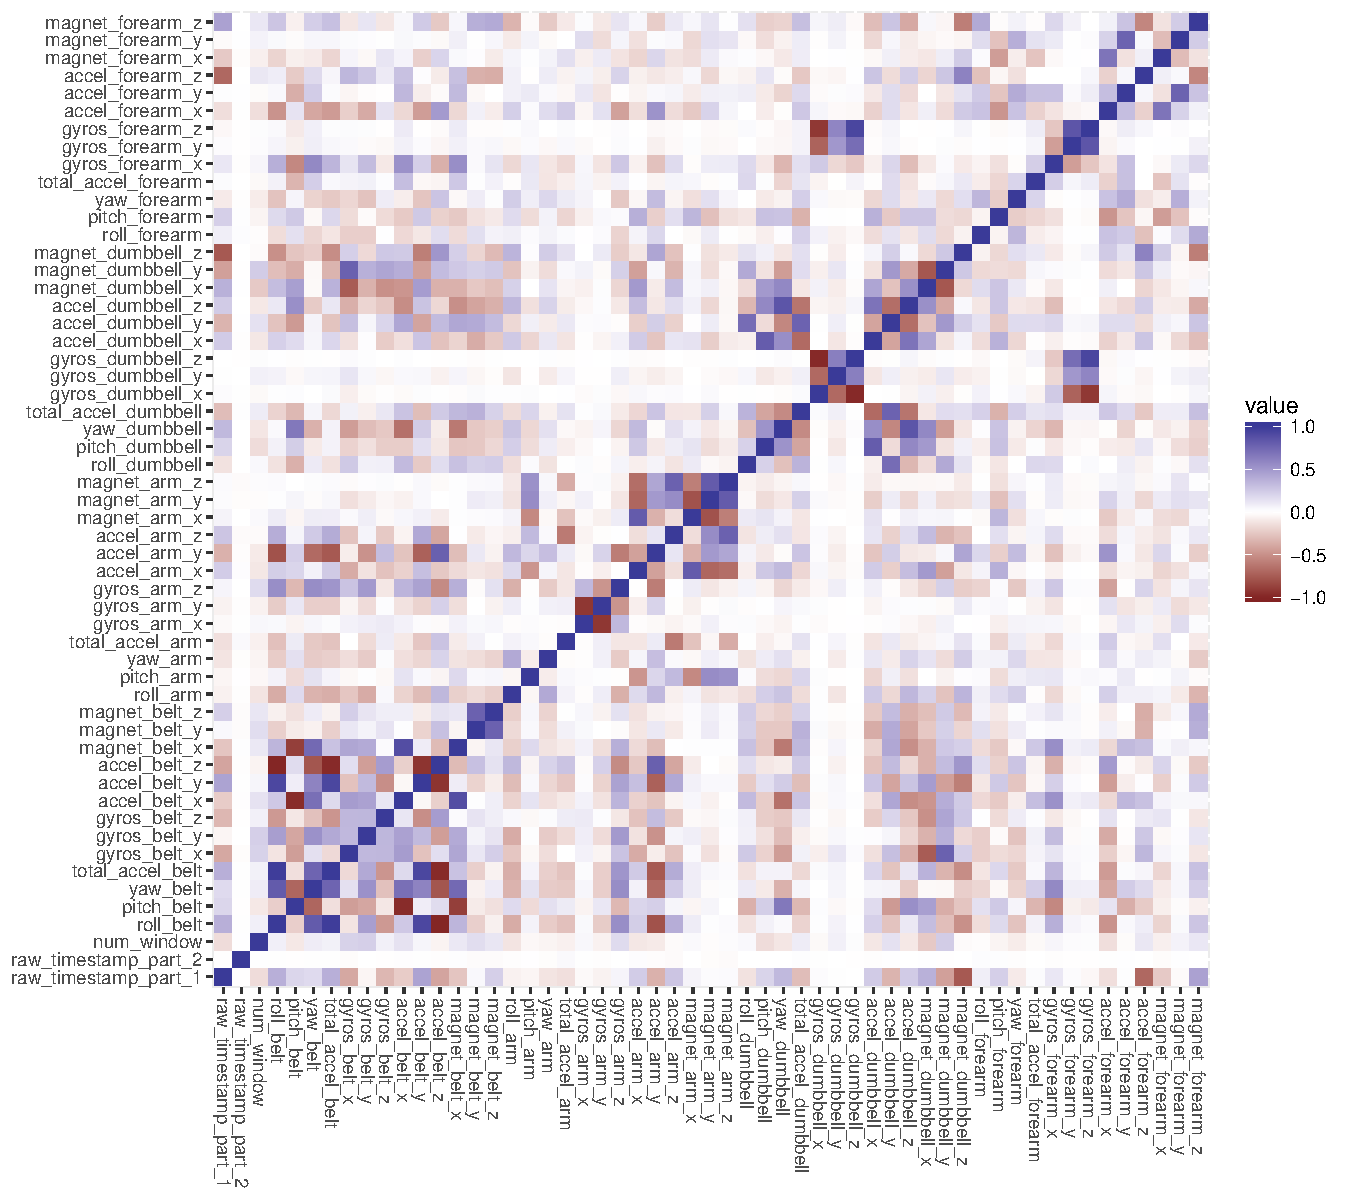
\includegraphics{Project_files/figure-latex/unnamed-chunk-6-1.pdf}

There seems to be strong correlation among variables in the bottom left.
Remove variables with a correlation coefficient over 0.9.

\begin{Shaded}
\begin{Highlighting}[]
\NormalTok{high_cor <-}\StringTok{ }\KeywordTok{findCorrelation}\NormalTok{(}\KeywordTok{cor}\NormalTok{(train[}\KeywordTok{sapply}\NormalTok{(train, is.numeric)]), }\DataTypeTok{cutoff =}\NormalTok{ .}\DecValTok{9}\NormalTok{)}

\NormalTok{train <-}\StringTok{ }\NormalTok{train[, }\OperatorTok{-}\NormalTok{high_cor]}
\NormalTok{test <-}\StringTok{ }\NormalTok{test[}\OperatorTok{-}\NormalTok{high_cor]}
\end{Highlighting}
\end{Shaded}

Slice the train data with 70\% as train set and 30\% as test set for
cross validation.

\begin{Shaded}
\begin{Highlighting}[]
\KeywordTok{set.seed}\NormalTok{(}\DecValTok{9999}\NormalTok{)}

\NormalTok{inTrain <-}\StringTok{ }\KeywordTok{createDataPartition}\NormalTok{(}\DataTypeTok{y =}\NormalTok{ train}\OperatorTok{$}\NormalTok{classe, }\DataTypeTok{p =} \FloatTok{0.7}\NormalTok{, }\DataTypeTok{list=}\OtherTok{FALSE}\NormalTok{)}
\NormalTok{trainSet <-}\StringTok{ }\NormalTok{train[inTrain, ]}
\NormalTok{testSet <-}\StringTok{ }\NormalTok{train[}\OperatorTok{-}\NormalTok{inTrain, ]}
\end{Highlighting}
\end{Shaded}

\section{Modeling}\label{modeling}

Use random forest algorithm with seven-fold cross validation as our
initial modeling method.

\begin{Shaded}
\begin{Highlighting}[]
\NormalTok{control <-}\StringTok{ }\KeywordTok{trainControl}\NormalTok{(}\DataTypeTok{method=}\StringTok{"cv"}\NormalTok{, }\DecValTok{7}\NormalTok{)}
\NormalTok{fit <-}\StringTok{ }\KeywordTok{train}\NormalTok{(classe }\OperatorTok{~}\StringTok{ }\NormalTok{., }\DataTypeTok{data =}\NormalTok{ trainSet, }\DataTypeTok{method =} \StringTok{"rf"}\NormalTok{, }\DataTypeTok{trControl =}\NormalTok{ control, }\DataTypeTok{ntree =} \DecValTok{250}\NormalTok{)}
\NormalTok{fit}
\end{Highlighting}
\end{Shaded}

\begin{verbatim}
## Random Forest 
## 
## 13737 samples
##    49 predictor
##     5 classes: 'A', 'B', 'C', 'D', 'E' 
## 
## No pre-processing
## Resampling: Cross-Validated (7 fold) 
## Summary of sample sizes: 11775, 11776, 11775, 11773, 11775, 11774, ... 
## Resampling results across tuning parameters:
## 
##   mtry  Accuracy   Kappa    
##    2    0.9867512  0.9832386
##   34    0.9973793  0.9966851
##   67    0.9965058  0.9955805
## 
## Accuracy was used to select the optimal model using the largest value.
## The final value used for the model was mtry = 34.
\end{verbatim}

Predict our random forest models on the test data from our original
train data and compute the out-of-sample error rate.

\begin{Shaded}
\begin{Highlighting}[]
\NormalTok{pred <-}\StringTok{ }\KeywordTok{predict}\NormalTok{(fit, testSet)}
\KeywordTok{confusionMatrix}\NormalTok{(pred, testSet}\OperatorTok{$}\NormalTok{classe)}
\end{Highlighting}
\end{Shaded}

\begin{verbatim}
## Confusion Matrix and Statistics
## 
##           Reference
## Prediction    A    B    C    D    E
##          A 1674    3    0    0    0
##          B    0 1136    0    0    0
##          C    0    0 1022    1    0
##          D    0    0    4  960    1
##          E    0    0    0    3 1081
## 
## Overall Statistics
##                                                
##                Accuracy : 0.998                
##                  95% CI : (0.9964, 0.9989)     
##     No Information Rate : 0.2845               
##     P-Value [Acc > NIR] : < 0.00000000000000022
##                                                
##                   Kappa : 0.9974               
##  Mcnemar's Test P-Value : NA                   
## 
## Statistics by Class:
## 
##                      Class: A Class: B Class: C Class: D Class: E
## Sensitivity            1.0000   0.9974   0.9961   0.9959   0.9991
## Specificity            0.9993   1.0000   0.9998   0.9990   0.9994
## Pos Pred Value         0.9982   1.0000   0.9990   0.9948   0.9972
## Neg Pred Value         1.0000   0.9994   0.9992   0.9992   0.9998
## Prevalence             0.2845   0.1935   0.1743   0.1638   0.1839
## Detection Rate         0.2845   0.1930   0.1737   0.1631   0.1837
## Detection Prevalence   0.2850   0.1930   0.1738   0.1640   0.1842
## Balanced Accuracy      0.9996   0.9987   0.9979   0.9974   0.9992
\end{verbatim}

The out-of-sample error rate for the cross-validation process is 0.998
and the out-of-sample error rate is only 0.002, which is pretty
competitive. Use the model as our final model.

\section{Prediction}\label{prediction}

Predict on the original test data set and print the result.

\begin{Shaded}
\begin{Highlighting}[]
\NormalTok{pred.val <-}\StringTok{ }\KeywordTok{predict}\NormalTok{(fit, test)}
\NormalTok{pred.val}
\end{Highlighting}
\end{Shaded}

\begin{verbatim}
##  [1] B A B A A E D B A A B C B A E E A B B B
## Levels: A B C D E
\end{verbatim}

\newpage

\section{Appendix}\label{appendix}

Visualize classification tree from CART algorithm.

\begin{Shaded}
\begin{Highlighting}[]
\NormalTok{modfit_tree <-}\StringTok{ }\KeywordTok{train}\NormalTok{(classe }\OperatorTok{~}\StringTok{ }\NormalTok{., }\DataTypeTok{method=}\StringTok{"rpart"}\NormalTok{, }\DataTypeTok{data=}\NormalTok{trainSet)}
\KeywordTok{fancyRpartPlot}\NormalTok{(modfit_tree}\OperatorTok{$}\NormalTok{finalModel)}
\end{Highlighting}
\end{Shaded}

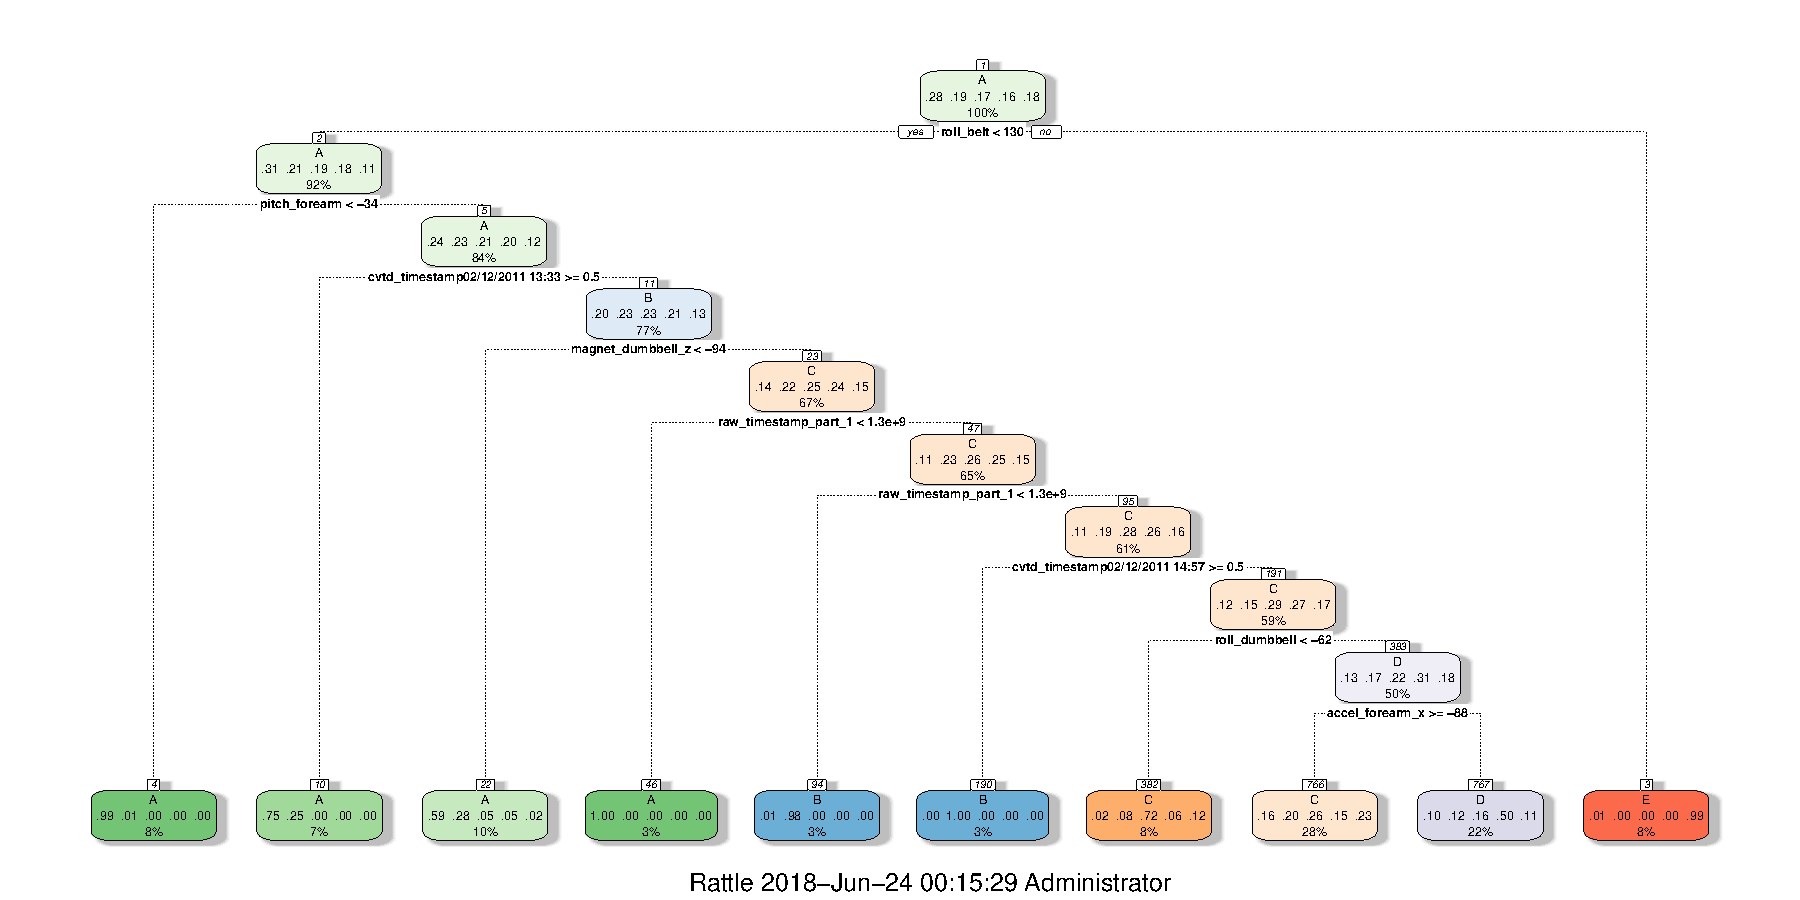
\includegraphics{Project_files/figure-latex/unnamed-chunk-12-1.pdf}


\end{document}
